\documentclass[tikz,border=12pt]{standalone}
\usepackage{amsmath}
\usetikzlibrary{arrows.meta}

\begin{document}
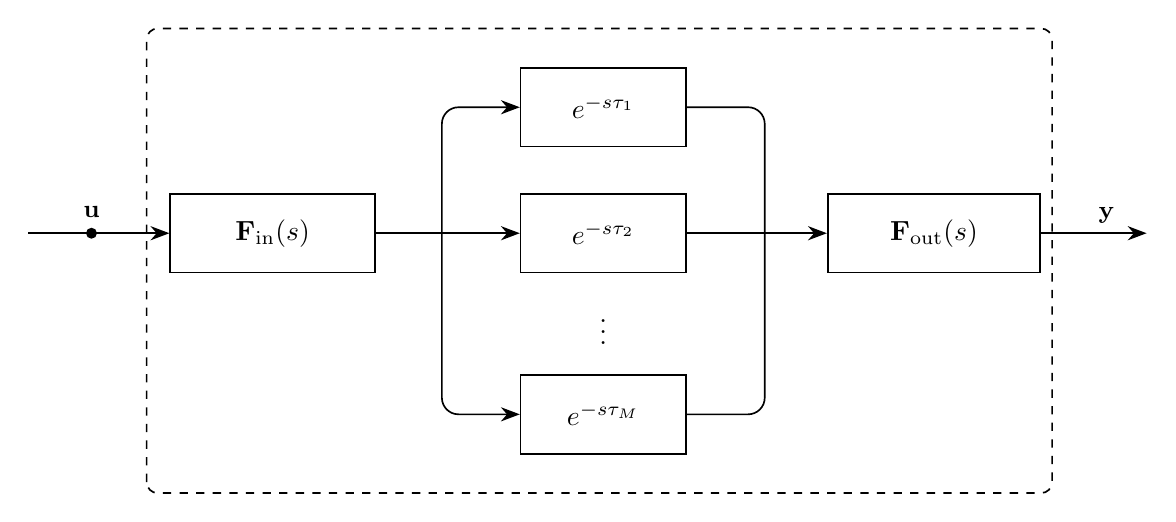
\begin{tikzpicture}[
    >={Stealth[length=2.4mm]},
    line/.style   = {semithick, rounded corners=6pt},
    block/.style  = {draw, semithick, fill=white,
                     minimum height=1cm, minimum width=2.3cm},
    signal/.style = {circle, fill, inner sep=1.4pt, label distance=3pt},
    sig/.style    = {font=\small}
]

% Three-block current propagation: StateSpace -> scalar modal delays -> StateSpace
\node[block, minimum width=2.6cm] (Fin)  at (-3.5, 0) {$\mathbf{F}_{\mathrm{in}}(s)$};
\node[block, minimum width=2.7cm] (Fout) at ( 4.9, 0) {$\mathbf{F}_{\mathrm{out}}(s)$};

\foreach \i/\lab/\y in {1/1/1.6, 2/2/0, N/M/-2.3}
    \node[block, minimum width=2.1cm] (D\i) at (0.7, \y) {$e^{-s\tau_{\lab}}$};
\node at (0.7, -1.15) {$\vdots$};

% Fan-out from a single internal point
\coordinate (split) at (-1.35, 0);
\draw[->, line] (-6.6, 0) -- (Fin.west);
\draw[line] (Fin.east) -- (split);
\draw[->, line] (split) -- (D2.west);
\foreach \b in {D1, DN}
    \draw[->, line] (split) |- (\b.west);

% Fan-in to the output state-space factor
\coordinate (join) at (2.75, 0);
\draw[line] (D2.east) -- (join);
\foreach \b in {D1, DN}
    \draw[line] (\b.east) -| (join);
\draw[->, line] (join) -- (Fout.west);
\draw[->, line] (Fout.east) -- (7.6, 0) node[sig, pos=0.62, above] {$\mathbf{y}$};

% Signal node: u external
\node[signal, label={[sig]above:$\mathbf{u}$}] at (-5.8, 0) {};

% Model enclosure
\draw[dashed, semithick, rounded corners=4pt] (-5.1, -3.3) rectangle (6.4, 2.6);

\end{tikzpicture}
\end{document}
